\documentclass[tikz]{standalone}

\usepackage{tikz}
\usepackage[svgnames]{xcolor}
\usepackage{tikz-3dplot}
\usepackage{amsmath} %математические формулы
\usepackage[e]{esvect}  %Красивая стрелочка вектора



\usetikzlibrary{calc}
\usetikzlibrary{arrows.meta}
\usetikzlibrary{angles}



\input{../tikzcom.tex}

\begin{document}
	
    
	     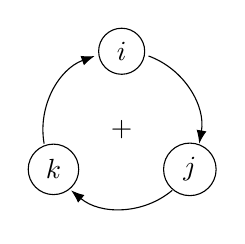
\begin{tikzpicture}[ scale=1]
	
			\draw node{$+$};
			
			\draw (90:1) node [circle, draw] {$i$};
			\draw ({90-120}:1) node [circle, draw] {$j$};
			\draw ({90-240}:1) node [circle, draw] {$k$};
			
			\draw [-Latex] (90-20:1) arc(90-20:90-120+20:1);
			\draw [-Latex] (90-120-20:1) arc(90-120-20:90-120-120+20:1);
			\draw [-Latex] (90-240-20:1) arc(90-240-20:90-120-240+20:1);
		
	    \end{tikzpicture} 
	    
	    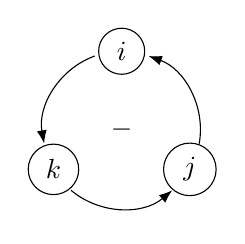
\begin{tikzpicture}[ scale=1]
	    	
	    	\draw node{$-$};
	    	
	    	\draw (90:1) node [circle, draw] {$i$};
	    	\draw ({90-120}:1) node [circle, draw] {$j$};
	    	\draw ({90-240}:1) node [circle, draw] {$k$};
	    	
	    	\draw [Latex-] (90-20:1) arc(90-20:90-120+20:1);
	    	\draw [Latex-] (90-120-20:1) arc(90-120-20:90-120-120+20:1);
	    	\draw [Latex-] (90-240-20:1) arc(90-240-20:90-120-240+20:1);
	    	
	    \end{tikzpicture} 

	
	
	
	







	
\end{document}